\chapter{Clúpiter}
\label{chap:conceptos_basicos}

\lettrine{P}{ara} comprender el objetivo del proyecto y su propuesta de valor, primero es necesario entender las características del mismo, la justificación de las mismas, y el funcionamiento de sus componentes más primitivos.

\section{Nombre y Marca Corporativa}
Si bien este no es un elemento altamente importante en un proyecto de ingeniería como este, si que es conveniente y nunca está de más otorgarle personalidad mediante la creación de un nombre e isotipo para el mismo.

El nombre del clúster es \textbf{Clúpiter} (ClúPIter): una mezcla entre las palabras ``Clúster'' y el ``PI'' de la \acrlong{rpi}, que de forma muy conveniente recuerda en su segunda parte a Júpiter. Este es a su vez planeta del sistema solar junto con el (enano) Plutón, nombre del clúster del GAC\footnote{\url{http://pluton.dec.udc.es}}. Es cuanto menos paradógico que el cluster en miniatura sea Júpiter, y el real sea Plutón\dots

En cuanto a la marca del cluster, éste no puede quedar sin un logo, que se expone a continuación:

TODO AQUÍ VA EL ISOLOGO %% INSERTAR ISOLOGO

\section{Precedentes}
Existen multitud de amateurs y amantes de la informática que como proyecto personal deciden montar un clúster de \acrlong{rpi}s, entre los que por ejemplo se encuentran Jeff Geerling\footnote{\url{https://www.youtube.com/user/geerlingguy}}. Además, en el mundo académico también ha habido aproximaciones muy similares, destacando \textit{Wee Archie}, un mini-supercomputador muy similar al de este proyecto de mayor tamaño, que permite explicaciones algo más interesantes con sus pantallas de matriz de LED.

Como se puede leer en la página web del proyecto \cite{wee_archie_webpage}, este es un supercomputador del tamaño de una maleta, que al igual que Clúpiter, sirve para explicar el funcionamiento de su hermano mayor, el supercomputador ARCHER\footnote{\url{https://www.archer.ac.uk}}.

\section{Conceptos Básicos}
\subsection{Raspberry Pi 4 Model B}
Cada aproximadamente dos años, la Raspberry Pi Foundation saca una nueva versión de su compacto y más exitoso producto: la \acrlong{rpi}, o por sus siglas \acrshort{rpi}. Estos pequeños computadores vienen en diversos formatos de forma, pero el que ha catapultado esta plataforma al éxito ha sido el formato que denominan \textit{Standard}\footnote{85.6 mm × 56.5 mm}.

\begin{figure}[h!]
  \centering
  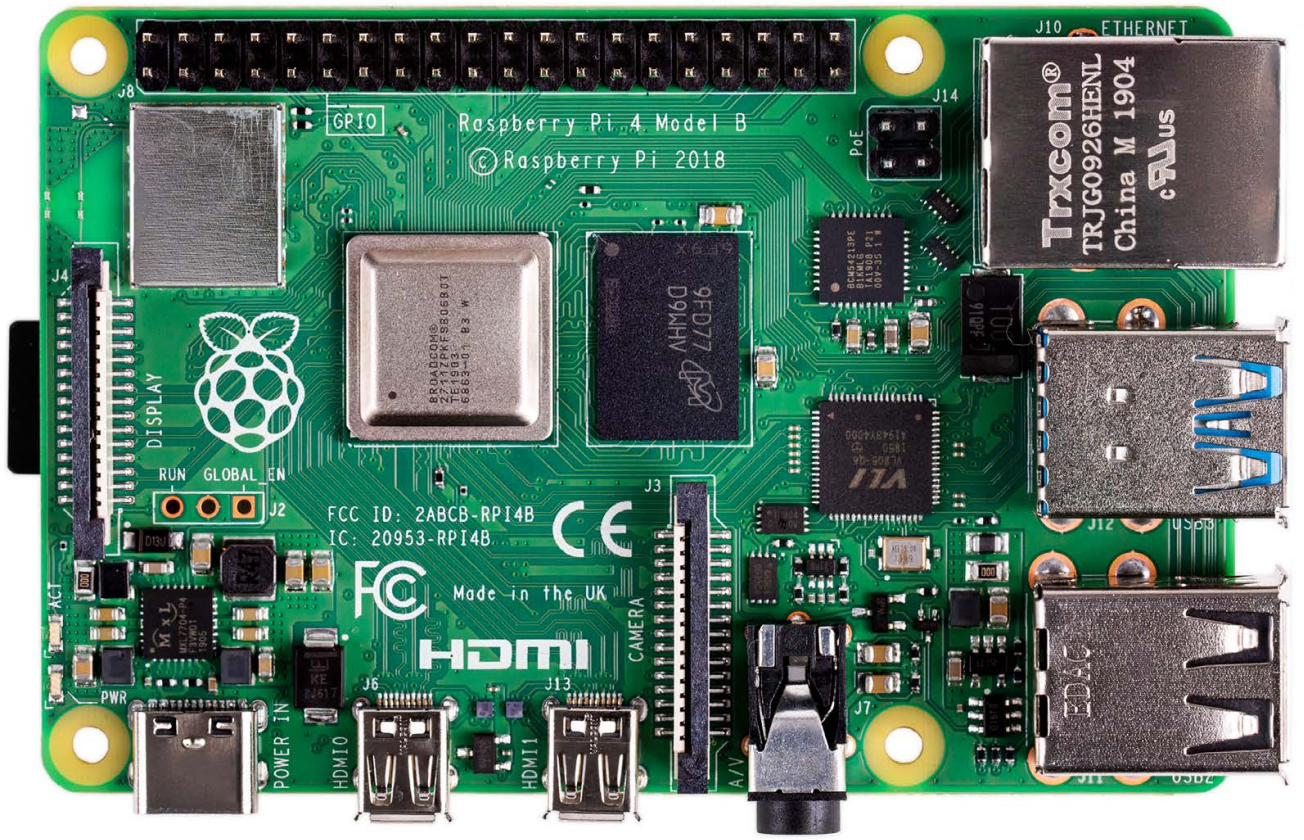
\includegraphics[width=0.75\textwidth]{img/rpi_parts/rpi_base.jpg}
  \caption{\acrlong{rpi} 4 Model B}
  \label{fig:rpi_base}
\end{figure}

Siendo cada versión mucho más potente que la anterior, y costando aproximadamente el mismo precio, está claro que la Raspberry Pi Foundation está haciendo un excelente trabajo aportando valor a este segmento del bajo consumo y coste.

La \acrlong{rpi} 4B (4 Model B) es la versión más nueva de formato standard, y por ello ha sido la elección para constituir la base del clúster. Las especificaciones de la misma son:

\subsubsection{CPU}
La CPU de este nuevo modelo es la \textbf{Broadcom BCM2711}, un procesador con arquitectura ARMv8-A y 4 núcleos Cortex-A72.

Estos núcleos cuentan con un \textit{pipeline} de 15 etapas, ejecución OOO (\textit{out-of-order}) y predictor de saltos, entre otros.

\begin{wrapfigure}[5]{r}{0.18\textwidth}
  \centering
  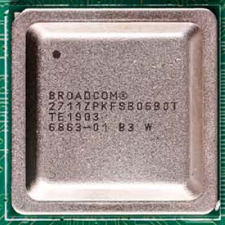
\includegraphics[width=0.18\textwidth]{img/rpi_parts/rpi_cpu.jpg}
  \label{fig:rpi_cpu}
\end{wrapfigure}
Además, cuenta con 48KB de L1I y 32KB de L1D por núcleo, así como 1MB de L2 compartido (256KB por núcleo). Esto emparejado con un único chip de 2GB de memoria LPDDR4-2400, es suficiente para un uso doméstico sencillo, pero quizás no sea la mejor disposición para el cómputo intensivo como se verá más adelante.
% TODO INSERTAR REF?????

\subsubsection{GPU/VPU}
A pesar de que el integrado que se muestra en la foto del apartado superior es un \acrshort{soc} (\textit{\acrlong{soc}}), se ha preferido tratar la CPU y la GPU/VPU por separado. Y es que los gráficos integrados de esta última \acrlong{rpi} son una importante mejora sobre la VideoCore IV que equipaban modelos anteriores.

La GPU en la \acrshort{rpi}4 es la VideoCore VI, y cuenta con multitud de soporte para multimedia y una potencia gráfica aceptable. En concreto, acelera por hardware H.265 (4Kp60 decode), H.264 (1080p60 decode, 1080p30 encode), y soporta OpenGL ES, 3.0.

\begin{wrapfigure}[8]{r}{0.35\textwidth}
  \centering
  
\includegraphics[width=0.35\textwidth]{img/vulkan_logo.png}
  \label{fig:vulkan_logo}
\end{wrapfigure}
Además, y lo que considero más interesante, es que posteriormente al lanzamiento se comenzó para esta gráfica el desarrollo de un driver de Vulkan: un estándar abierto de última generación para programación de gráficos, pero que también se puede emplear para cómputo. Esto es una fantástica noticia, ya que permite acelerar ciertas cargas de trabajo aprovechando la inmensa capacidad de cómputo paralelo de estos dispositivos, siendo una de las más habituales en estos dispositivos la transformada de Fourier.

Realizar algún tipo de programa para computación \acrshort{gpgpu} (\textit{\acrlong{gpgpu}}) en Vulkan queda fuera de lo que pretende abarcar este trabajo, pero es un interesante proyecto para la realización de alguna otra iteración sobre esta plataforma.

\subsubsection{E/S}
En términos de entrada/salida la \acrshort{rpi}4B cuenta con multitud de puertos. Los que se van a usar son Gigabit Ethernet y USB 3.0, sin embargo equipa de serie otros muchos ortos puertos en el \acrshort{gpio} (\acrlong{gpio}), como son DSI (\textit{Display Serial Interface}), CSI (\textit{Camera Serial Interface}), I2C (\textit{Inter-Integrated Circuit}), UART (\textit{Universal Asynchronous Receiver-Transmitter}), SPI (\textit{Serial Peripheral Interface}), y video compuesto, así como dos salidas HDMI.

\begin{figure}[h!]
  \centering
  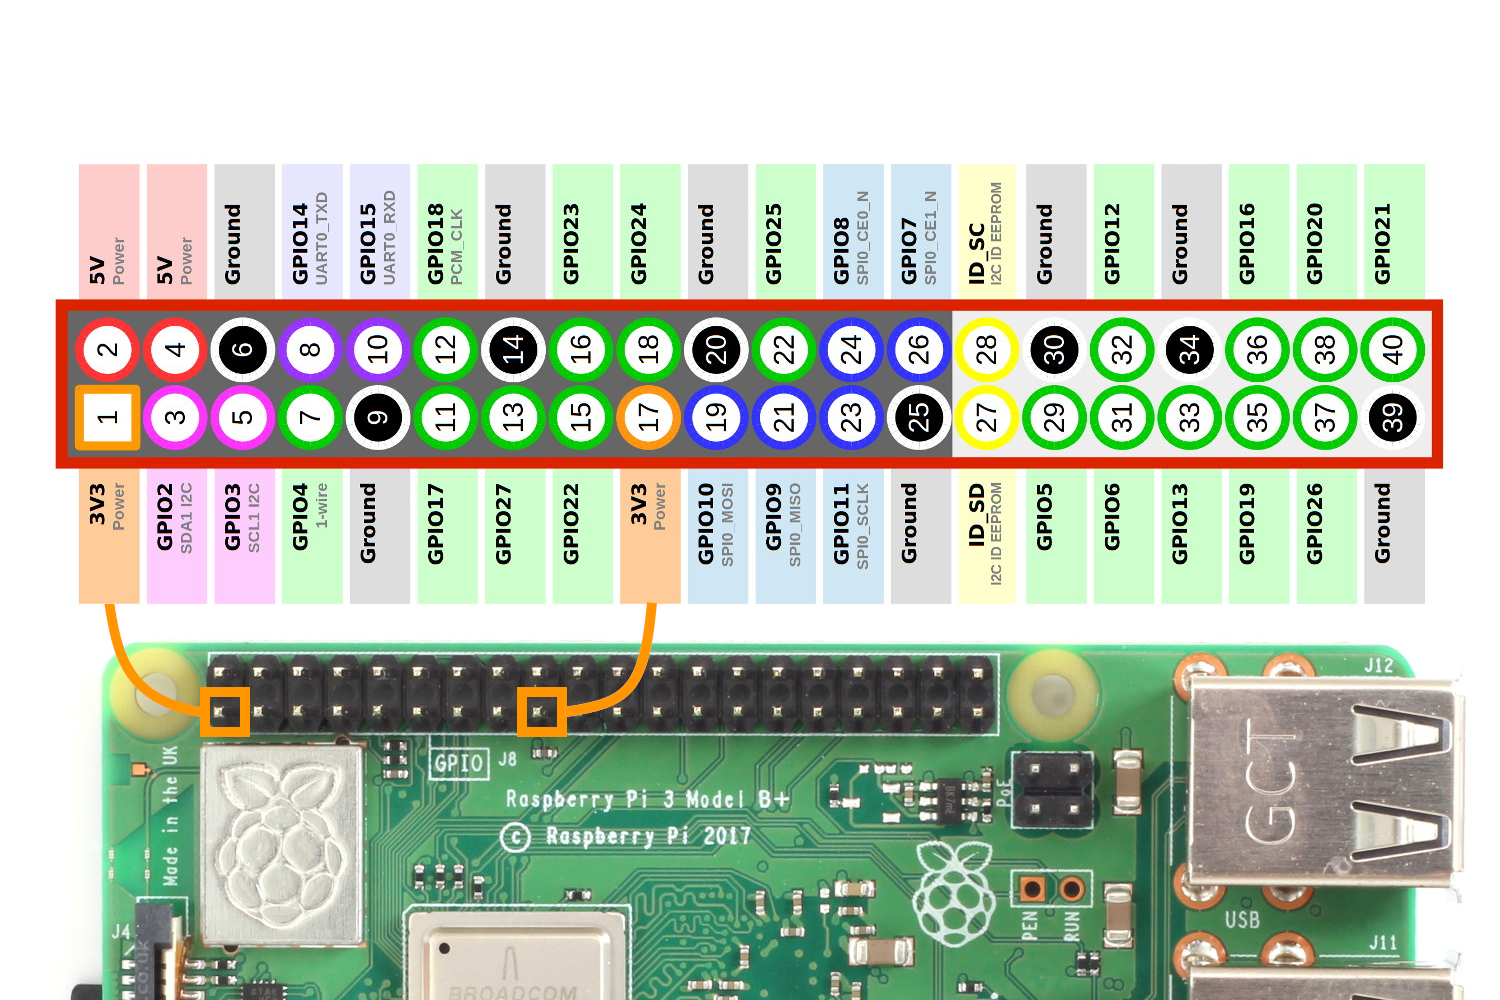
\includegraphics[width=0.85\textwidth]{img/rpi_parts/rpi_gpio.png}
  \caption{Pines GPIO de la \acrlong{rpi} 3, idénticos a los de la 4}
  \label{fig:rpi_gpio_pinout}
\end{figure}

\subsection{OpenMPI}
explicación openmpi